\documentclass{standalone}
\usepackage{tkz-fct}
\usepackage{tkz-euclide}
\usepackage{amsmath}
\usepackage{color}
\renewcommand*\familydefault{\sfdefault}
\usepackage{sansmath}
\sansmath
\renewcommand{\arraystretch}{2.6}
\definecolor{gray75}{gray}{0.75}
\begin{document}
 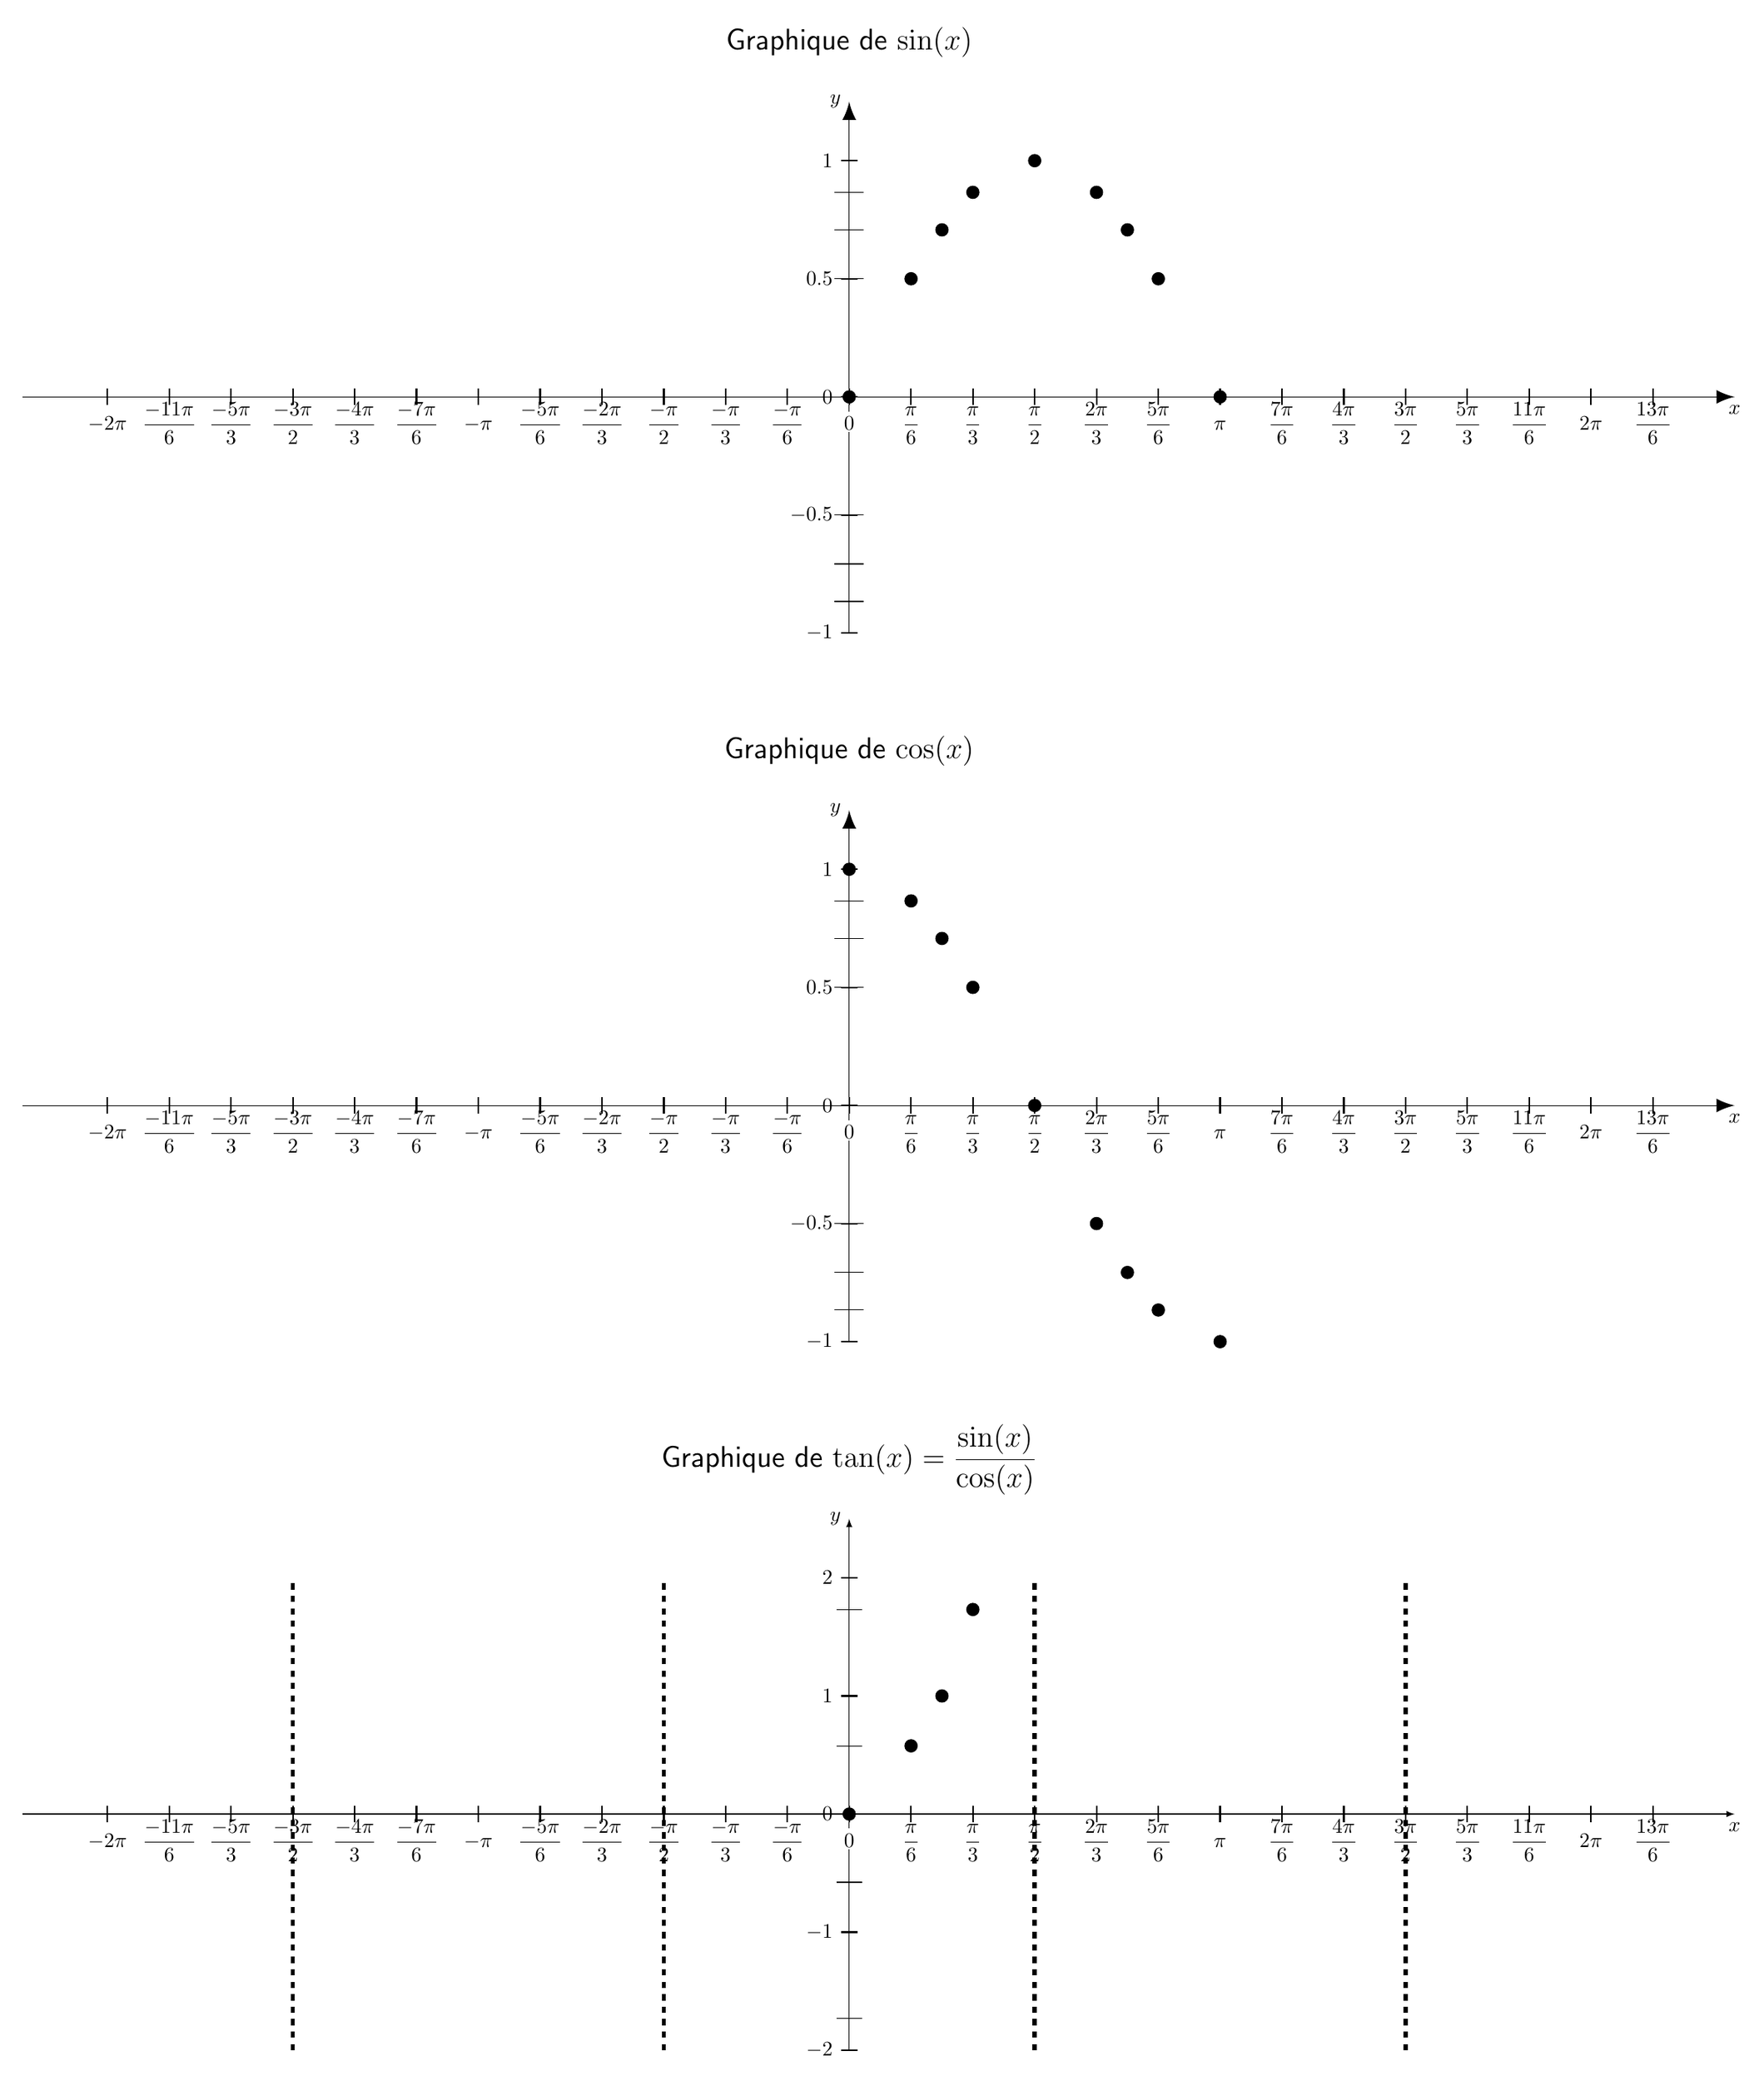
\begin{tikzpicture}[scale=2]
   \tkzInit[xmin=-7,xmax=7,ymin=-2,ymax=2, ystep=1]
\tkzAxeY
\tkzAxeX[trig=6]
 \tkzDefPoints{0/0.57735026919/S1,0/1.73205080757/S2,0/-0.57735026919/S3,0/-1.73205080757/S4}
   \tkzDrawPoints[shape=cross,size=12](S1,S2,S3,S4)

\foreach\v in {-3,-1,1,3}
{
  \tkzVLine[color=black, dashed, line width=2pt]{\v*\FPpi/2}
}
\foreach\v in {-5,-3,1,3}
{
\tkzFct[line width=2pt,domain=\v*\FPpi/2+0.2:(\v+2)*\FPpi/2-0.2]{tan(\x)}

}
\tkzFct[line width=2pt,domain=-\FPpi/2+0.2:\FPpi/2-0.2]{tan(\x)}
\foreach\v in {0,1,2}
{
\tkzDefPointByFct[]({\v*\FPpi/6})\tkzGetPoint{A}\tkzDrawPoint[size=6](A)
}
\foreach\v in {1}
{
\tkzDefPointByFct({\v*\FPpi/4})\tkzGetPoint{A}\tkzDrawPoint[size=6](A)
}
\tkzText(0,3){\Large Graphique de $\tan(x)=\dfrac{\sin(x)}{\cos(x)}$}

\begin{scope}[yshift=12cm]
   \tkzInit[xmin=-7,xmax=7,ymin=-1,ymax=1, ystep=0.5]
\tkzAxeY
\tkzAxeX[trig=6]
 \tkzDefPoints{0/0.5/S1,0/0.70710678118/S2,0/0.86602540378/S3}
   \tkzDrawPoints[shape=cross,size=12](S1,S2,S3)

      \tkzDefPoints{0/-0.5/S1,0/-0.70710678118/S2,0/-0.86602540378/S3}
   \tkzDrawPoints[shape=cross,size=12](S1,S2,S3)


\tkzFct[line width=2pt,domain=-7:7]{sin(\x)}

\foreach\v in {0,1,...,6}
{
\tkzDefPointByFct[]({\v*\FPpi/6})\tkzGetPoint{A}\tkzDrawPoint[size=6](A)
}
\foreach\v in {1,3}
{
\tkzDefPointByFct({\v*\FPpi/4})\tkzGetPoint{A}\tkzDrawPoint[size=6](A)
}
\tkzText(0,1.5){\Large Graphique de $\sin(x)$}
\end{scope}
\begin{scope}[yshift=6cm]
   \tkzInit[xmin=-7,xmax=7,ymin=-1,ymax=1, ystep=0.5]
\tkzAxeY
\tkzAxeX[trig=6]
 \tkzDefPoints{0/0.5/S1,0/0.70710678118/S2,0/0.86602540378/S3}
   \tkzDrawPoints[shape=cross,size=12](S1,S2,S3)

      \tkzDefPoints{0/-0.5/S1,0/-0.70710678118/S2,0/-0.86602540378/S3}
   \tkzDrawPoints[shape=cross,size=12](S1,S2,S3)


\tkzFct[line width=2pt,domain=-7:7]{cos(\x)}
\foreach\v in {0,1,...,6}
{
\tkzDefPointByFct[]({\v*\FPpi/6})\tkzGetPoint{A}\tkzDrawPoint[size=6](A)
}
\foreach\v in {1,3}
{
\tkzDefPointByFct({\v*\FPpi/4})\tkzGetPoint{A}\tkzDrawPoint[size=6](A)
}
\tkzText(0,1.5){\Large Graphique de $\cos(x)$}

\end{scope}
 \end{tikzpicture}

\end{document}
